\chapter{\textbf{THEORY FRAMEWORK}}
In this chapter, we present the theoretical background underpinning the study, commencing with an introduction to the tight-binding method as the main approach to describe the electronic structure of \acp{TMD}. The crystal structure of \acp{TMD} is also discussed to determine their symmetries. Additionally, in the presence of a magnetic field, electronic motion becomes quantized into Landau levels, as first proposed by Lev Landau. Following this, we also present the theoretical framework of the Hall effect, beginning with the classical Hall effect and culminating with the quantum Hall effect, as presented in Ref.~\cite{klitzing90}. The study of Hall effect based largely on the treatment in Ref.~\cite{xiao2010berry}.


\section{The tight-binding method}\label{Section 2.1}
The tight-binding approximation is based on the \ac{LCAO} method. This approach constructs electronic wave functions using the atomic orbitals of isolated atoms. In the tight-binding method, we assume the electrons stay close to the atomic sites and the overlap between neighboring orbitals is small.\\
We start with the single electron time-indepentdent Schr\"{o}dinger equation
\begin{gather}
	H_{\text{1e}} \psi = \left[-\f{\hbar^{2} \nabla^{2}}{2m} + U_{0}(\mathbf{r})\right] \psi_{\lambda,\mathbf{k}}(\mathbf{r}) = \varepsilon_{\lambda}(\mathbf{k}) \psi_{\lambda,\mathbf{k}}(\mathbf{r}),
\end{gather}
where $U_{0}(\mathbf{r})$ is the periodic lattice potential, $\psi_{\lambda,\mathbf{k}}(\mathbf{r})$ is the Bloch wavefunction of an electron in band $\lambda$ with wave vector $\mathbf{k}$ and $\varepsilon_{\lambda}(\mathbf{k})$ is the energy dispersion in crystal. In the \ac{LCAO} method, the electronic wave function can be written as 
\begin{gather}
	\psi_{\text{LCAO}} = \frac{1}{\sqrt{N}}\sum_{n = 1}^{N} \sum_{i = 1}^{N_{i}} \sum_{j = 1}^{N_{\text{orb}}} c_{j,i}(\mathbf{R}_{n}) \phi_{j} (\mathbf{r} - \mathbf{R}_{n} - \mathbf{r}_{i}),
\end{gather}
in which $\phi_{j}$ is the orbital wave function $j$ of an atomic $i$ localized on a lattice site $\mathbf{R}_{n}$. Here, $ N_{\text{orb}} $ is the number of orbitals per atom, $ N_{i} $ is the number of atoms in the unit cell, and $ N $ is the number of unit cells.

As for the \acf{TBM} and the \ac{LCAO} theory, the single electron Bloch wave function can be expressed in terms of atomic orbitals as follows
\begin{gather}
	\psi_{\lambda,\mathbf{k}}(\mathbf{r}) = \frac{1}{\sqrt{N}} \sum_{n=1}^{N} \sum_{i = 1}^{N_{i}} \sum_{j = 1}^{N_{\text{orb}}} C_{j,i}^{\lambda} (\mathbf{k})  e^{i \mathbf{k} (\mathbf{R_{n}} + \mathbf{r}_{i})} \phi_{j} (\mathbf{r} - \mathbf{R}_{n} - \mathbf{r}_{i}) ,
\end{gather}
here, $C_{ji}^{\lambda}(\mathbf{k})$ are the coefficients of linear expansion.

Thanks to the wave function found in Eq.~(2.2), now we apply $e^{-i \mathbf{k} \cdot \mathbf{r}_{i'}} \phi_{j'}^{*}(\mathbf{r} - \mathbf{r}_{i'})$ to the left of the single electron Schr\"{o}dinger Eq.~(2.1) and taking the sum over $\mathbf{r}$
\begin{gather}
	\sum_{i = 1}^{N_{i}} \sum_{j = 1}^{N_{\text{orb}}} \left( H_{j' i', j i}(\mathbf{k}) - \varepsilon(\mathbf{k}) S_{j' i', j i}(\mathbf{k}) \right) C_{j,i}^{\lambda}(\mathbf{k}) = 0,
\end{gather}
where
\begin{gather}
	H_{ji,ji}(\mathbf{k}) =  \int \phi_{j}^{*}(\mathbf{r} - \mathbf{r}_{i}) H_{1\text{e}} \phi_{j}({\mathbf{r} - \mathbf{r}_{i}}),
\end{gather}
is the on-site energy,
\begin{gather}
	H_{j'i',ji}(\mathbf{k}) =  \sum_{n = 1}^{N} e^{i \mathbf{k} \cdot (\mathbf{R}_{n} + \mathbf{r}_{i} - \mathbf{r}_{i'})} \int \phi_{j'}^{*}(\mathbf{r} - \mathbf{r}_{i'}) H_{1\text{e}} \phi_{j}({\mathbf{r} - \mathbf{R}_{n} - \mathbf{r}_{i}}),
\end{gather}
is the hopping energy,
\begin{gather}
	S_{j'i',ji}(\mathbf{k}) =  \sum_{n = 1}^{N} e^{i \mathbf{k} \cdot (\mathbf{R}_{n} + \mathbf{r}_{i} - \mathbf{r}_{i'})} \int \phi_{j'}^{*}(\mathbf{r} - \mathbf{r}_{i'})  \phi_{j}({\mathbf{r} - \mathbf{R}_{n} - \mathbf{r}_{i}}),
\end{gather}
is the overlap integral. 
The terms $H_{j'i',ji}$ and $H_{ji,ji}$ are called the Hamiltonian matrix elements. The solution of the Eq.~(2.4) is the eigenvalue $\varepsilon$ of the Schr\"{o}dinger Eq.~(2.1). Each eigenvalue give an energy dispersion of the system, called the energy band. 

The term in Eq.~(2.6) is often referred to as the \emph{hopping parameter}, which characterizes the strength of the interaction between atoms at positions $ i $ and $ i' $. A larger value implies stronger bonding and easier electron transfer between the atoms. In tight-binding theory, these matrix elements are often obtained from experimental data and treated as semi-empirical parameters.
\section{Crystal structure of TMDs}

\begin{figure}[H]
	\centering
	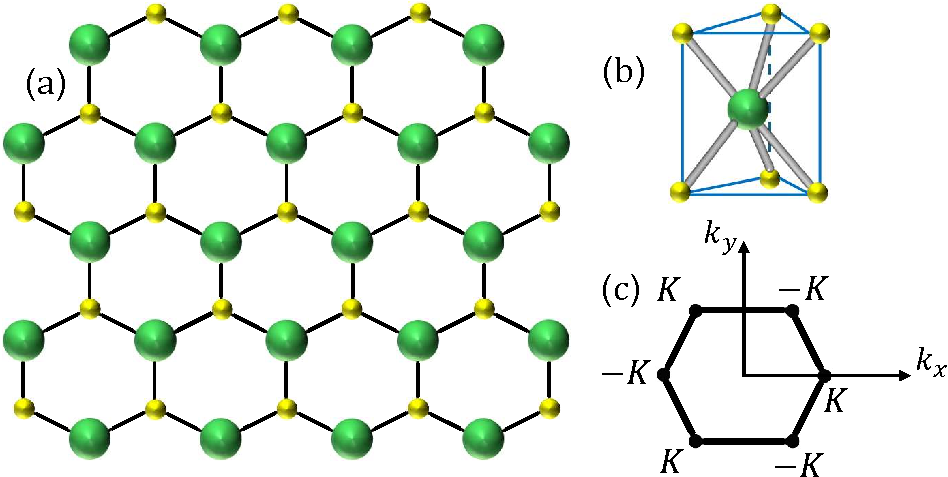
\includegraphics[width=\linewidth]{pic/latticePresent.pdf}
	\caption[Structure of TMD.]{\label{fig:Lattice}Structure of TMD. (a) Top view of monolayer MX$_{2}$. (b) sideview of monolayer MX$_{2}$. The green spheres represent M atoms, which are sandwiched by two layer of X atoms (yellow spheres). (c) The first Brillouin zone and high symmetry points in $k$-space.}
\end{figure}
Monolayer \acp{TMD} are \ac{2D} materials composed of transition metal and chalcogen atoms arranged in a honeycomb lattice, as illustrated in Fig.~2.1. These materials exhibit $D_{3h}$ point group symmetry \cite{mattheiss1973}. It were first studied in their buld forms as early as the 1960s, mainly in the context of solid-state and materials science. However, scientists moved their interested in monolayer TMDs, i.e, their \ac{2D} form, began to grow significantly after the isolation of graphene in 2004.

In monolayer \acp{TMD}, each transition metal (M) atom contributes five $d$-orbitals: $d_{z^{2}}$, $d_{x^{2} - y^{2}}$, $d_{xy}$, $d_{xz}$, and $d_{yz}$, while each chalcogen (X) atom contributes three $p$-orbitals: $p_{x}$, $p_{y}$, and $p_{z}$. The transition metal atoms form a triangular lattice and are sandwiched between two layers of chalcogen atoms, which themselves are arranged on a triangular lattice at alternating hollow sites. This arrangement results in a trigonal prismatic coordination, where each metal atom is surrounded by six chalcogen atoms positioned at the vertices of a trigonal prism, as shown in Fig.~2.1(b). The top view of monolayer \acp{TMD} is shown in Fig.~2.1(a). The Bravais lattice is spanned by the basis vectors
\begin{gather}
	\vv{a}_{1} = (a,0,0), \vv{a}_{2} = \left( \frac{a}{2}, \frac{\sqrt{3}}{2}a,0 \right),
\end{gather}
where $a$ is lattice constant. The first Brillouin zone of the \ac{TMD} is hexagonal with the high-symmetry points are defined as follows: $\Gamma = (0,0), K = (\tfrac{4\pi}{3a},0)$ and $M = (\tfrac{\pi}{a}, \tfrac{\pi}{\sqrt{3}a})$.





\section{Landau level in magnetic field}
The concept of Landau levels was first introduced by Lev Landau in 1930, describing the quantization of electronic motion in a two-dimensional electron gas under a perpendicular magnetic field. In this section, we briefly revisit the derivation of the Landau level spectrum from the single-particle Hamiltonian, providing a general theoretical overview that lays the foundation for the more complex tight-binding calculations presented later in this thesis.

We begin with the single particle Hamiltonian
\begin{gather}
	H = \frac{\mathbf{p}^{2}}{2m},
\end{gather}
where we apply the substitution
\begin{gather}
	\mathbf{p} \to \mathbf{p} = \boldsymbol{\Pi} + e \mathbf{A}(\mathbf{r}),
\end{gather}
with $\mathbf{A}(\mathbf{r})$ specified in the Landau gauge as $\mathbf{A} = (0, Bx, 0)$. The Hamiltonian then becomes
\begin{equation}
	\begin{aligned}
		H &= \frac{1}{2m} \left(\boldsymbol{\Pi} + e\mathbf{A}(\mathbf{r})\right)^2 \\
		&= \frac{\Pi_{x}^{2}}{2m} + \frac{(\Pi_{y} + eBx)^2}{2m}.
	\end{aligned}
\end{equation}

To diagonalize this Hamiltonian, we define the following ladder operators
\begin{equation}
	\begin{aligned}
		a &= \sqrt{\frac{1}{2\hbar eB}} \left(\Pi_{x} + i \Pi_{y}\right), \\
		a^{\dagger} &= \sqrt{\frac{1}{2\hbar eB}} \left(\Pi_{x} - i \Pi_{y}\right), \\
		b &= \sqrt{\frac{eB}{2\hbar}} \left(y - \frac{1}{eB} \Pi_{x} + i x\right), \\
		b^{\dagger} &= \sqrt{\frac{eB}{2\hbar}} \left(y - \frac{1}{eB} \Pi_{x} - i x\right).
	\end{aligned}
\end{equation}
The inverse transformations read
\begin{equation}
	\begin{aligned}
		\Pi_{x} &= \sqrt{\frac{\hbar eB}{2}} (a + a^{\dagger}), \\
		\Pi_{y} &= i\sqrt{\frac{\hbar eB}{2}} (a^{\dagger} - a).
	\end{aligned}
\end{equation}
The operators $a$ and $a^{\dagger}$ satisfy the bosonic commutation relation
\begin{gather}
	[a, a^{\dagger}] = 1, \quad [a, a] = [a^{\dagger}, a^{\dagger}] = 0.
\end{gather}
Operators $b$ and $b^{\dagger}$ also obey:
\begin{gather}
	[b, b^{\dagger}] = 1, \quad [b, b] = [b^{\dagger}, b^{\dagger}] = 0,
\end{gather}
and in addition, the $a$ and $b$ sectors commute:
\begin{gather}
	[a, b] = [a, b^{\dagger}] = [a^{\dagger}, b] = [a^{\dagger}, b^{\dagger}] = 0.
\end{gather}

As in the one-dimensional harmonic oscillator, the ladder operators act as
\begin{equation}
	\begin{aligned}
		a \ket{n} = \sqrt{n} \ket{n-1}, \quad a^{\dagger} \ket{n} = \sqrt{n+1} \ket{n+1},
	\end{aligned}
\end{equation}
where $\ket{n}$ is an eigenstate of the number operator $a^{\dagger}a$ with eigenvalue $n \geq 0$.

The Hamiltonian in Eq.~(2.11) can now be written in terms of $a$ and $a^{\dagger}$ as
\begin{gather}
	H = \hbar \omega_c \left(a^{\dagger} a + \frac{1}{2}\right), \quad \text{with } \omega_c = \frac{eB}{m}.
\end{gather}
The eigenvalues of Eq.~(2.18) are known as \acp{LL}
\begin{gather}
	E_{n} = \left(n + 1/2\right) \hbar \omega_{c},
\end{gather}
where $n$ is the Landau level index and $\omega_{c}$ is called the cyclotron frequency. These quantized energy are known as \acp{LL}. Each level labeled by the index $n$. The Fig.~2.2 illustrates the Landau level energy spectrum as a function of magnetic field strength. Each line represents a discrete energy level labeled by the Landau index $n$. As the magnetic field $B$ increases, the spacing between adjacent grows linearly due to the dependence of the cyclotron frequency $\omega_{c}$. At zero field, the spectrum is continous, corresponding to the free electron case. However, in the presence of magnetic field, the energy is quantized into discrete levels, leading to the characteristic ladder-like structure shown in the figure.

\begin{figure}[H]
	\centering
	\includegraphics[width=0.5\linewidth]{pic/LLDEMO.pdf}
	\caption[Landau levels.]{Representation of the Landau levels of Eq.~2.19.}
\end{figure}

%These levels give rise to what is called ``the Landau fan'', being very important in the de Haas-van Alphen and Shubnikov-de Haas effects \cite{10.1119/1.1615568} which predicts oscillations of the magnetic moment of a meltal depending on an applied magnetic field.


%More interesting is the top and bottom of conduction and valence band of the zero field spectrum. This results in a non-standard Landau levels when the field is turned on, as discused above.\\
%In the one-band case, knowing the effective mass in zero field and the charge is enough to determine the Landau level spectruc to linear order in the magnetic field. For the three-band case
%
%
% In order to determine the cyclotron frequency for the three-band, through the derivation in Appendix C, we have obtained the Landau levels for the three-band model when the field is turned on
%\begin{figure*}[htb]
%	\centering
%	\begin{subfigure}[b]{0.49\textwidth}
%		\centering
%		{\includegraphics[width=0.85\textwidth,height=1.2\linewidth]{pic/small_area_LL_3band.png}}
%	\end{subfigure}
%	\begin{subfigure}[b]{0.49\textwidth}
%		\centering
%		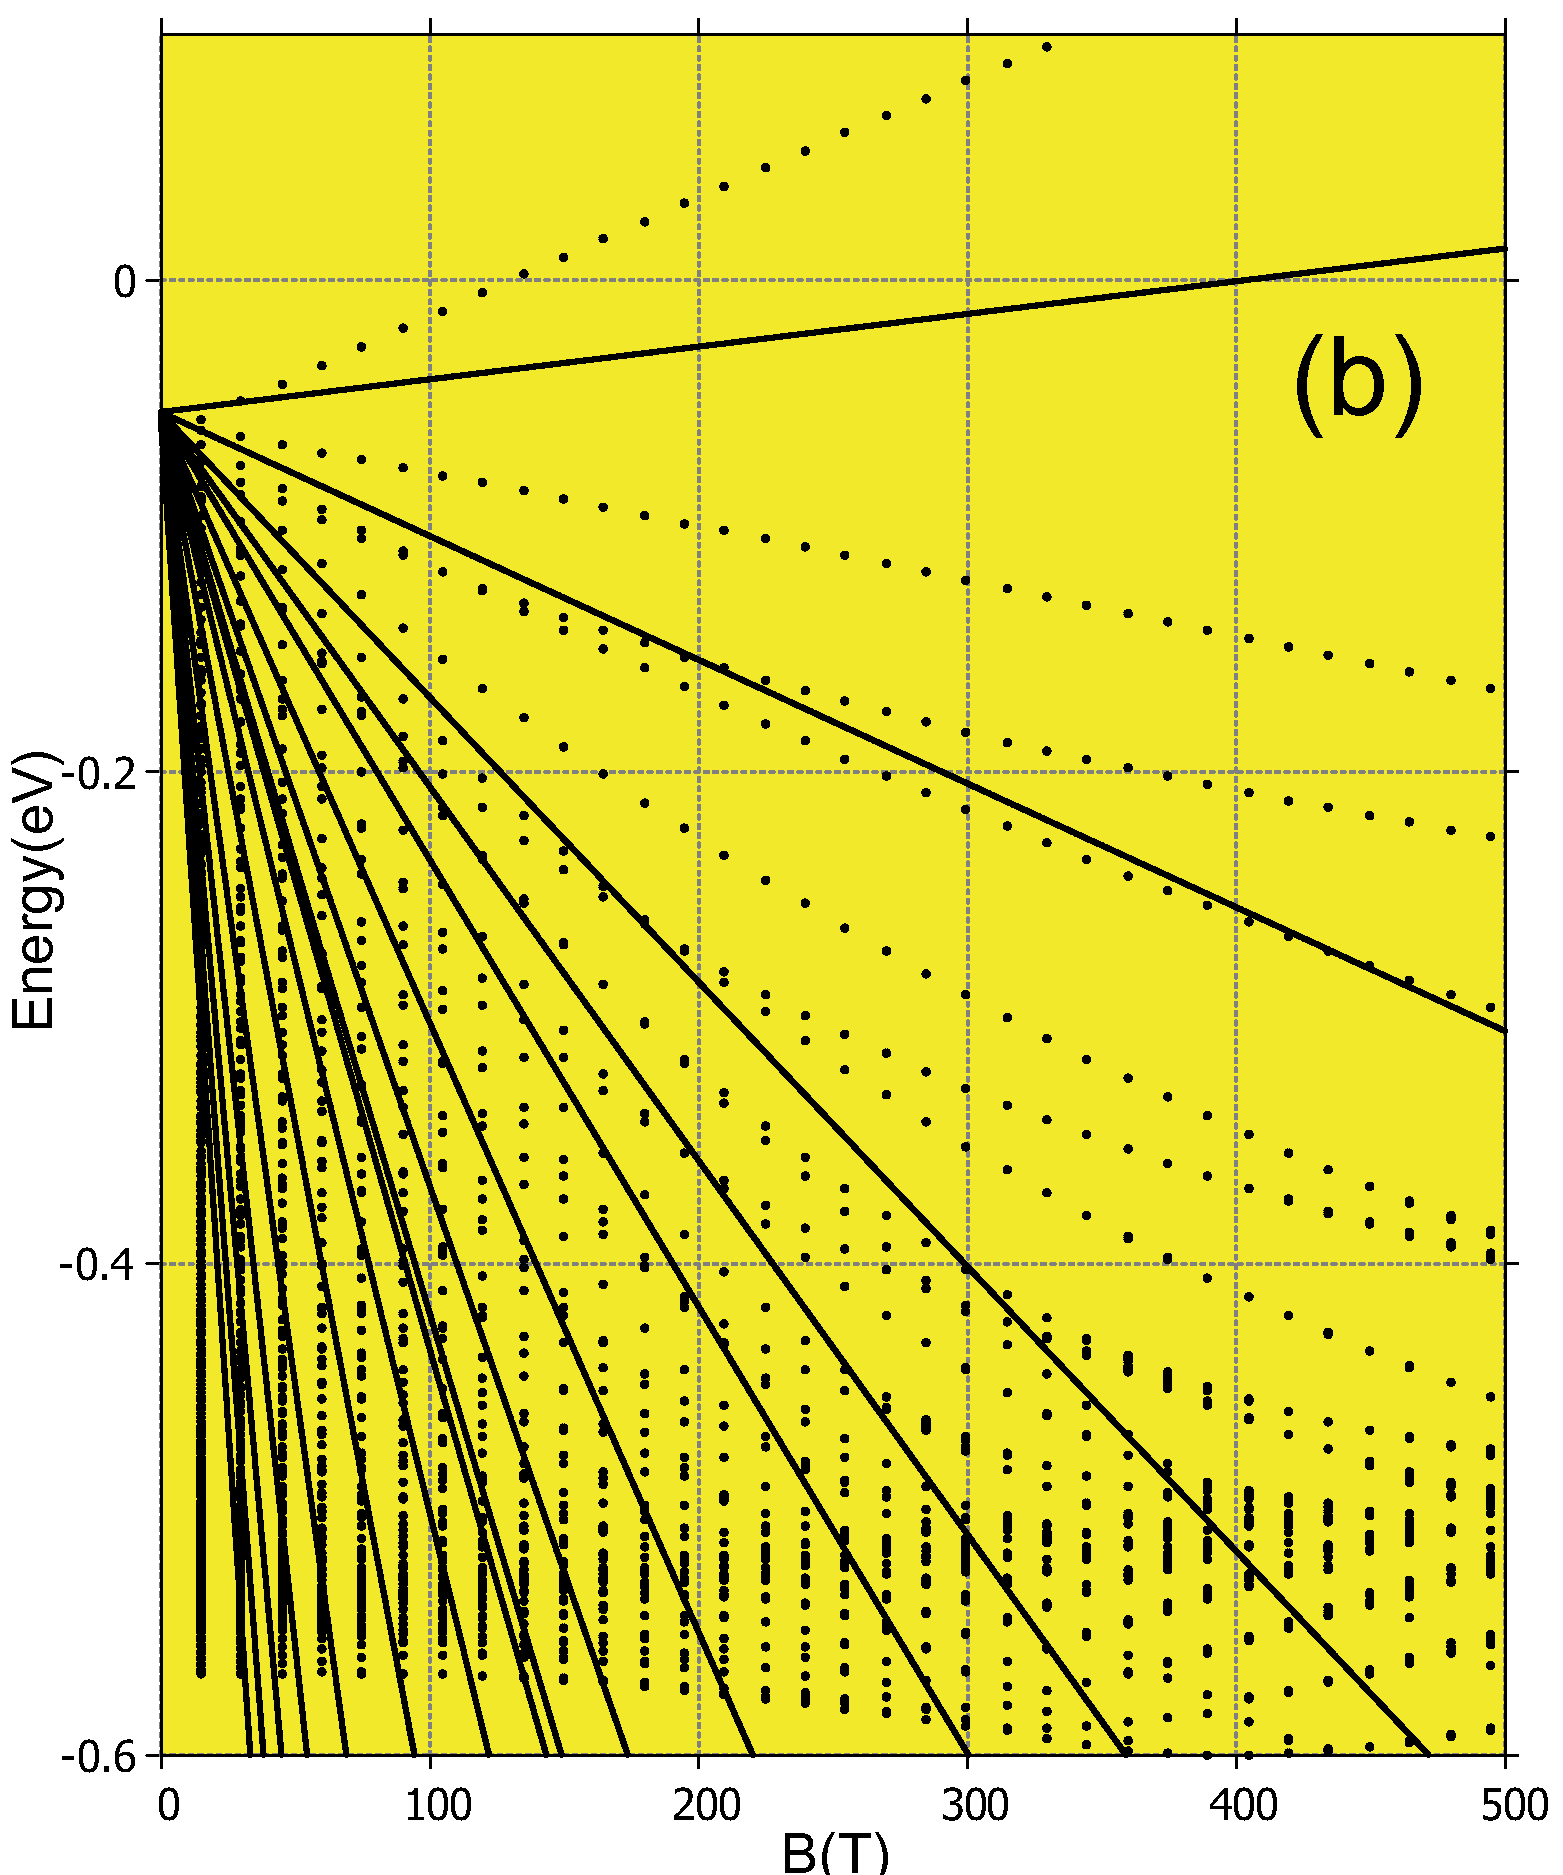
\includegraphics[width=0.85\textwidth,height=1.2\linewidth]{pic/landaulevel_3band_q_797_EF_final.pdf}
%	\end{subfigure}
%	\caption{
%		test
%	}
%\end{figure*}
%Ta có thể thấy một số mức Landau có năng lượng là được tăng tuyến tính theo cường độ từ trường, nhưng lại không cách đều và chính xác như hình của Hofstadter butterfly. Thêm vào đó có nhiều trạng thái mà năng lượng tại đó thì giảm trong khi đó thì từ trường lại tăng. những trạng thái này sẽ được gọi là những trạng thái ``kì cục'' mà ta sẽ bàn luận ở đây.\\
%Trong trường hợp một band, khối lượng hiệu dụng $m^{*}$ và điện tích là đủ để mô tả được phổ Landau theo sự thay đổi tuyến tính của từ trường. Trong trường hợp 2 band và 3 band thì


%It is this fan of Landau levels that responsible for the de Haas-van Alphen and Shubnikov-de Haas effects.

\section{Hall effect}
\subsection{The classical Hall effect}

Before delving into the quantum Hall effect, let us start by taking a look at its classical counterpart i.e., the Hall effect. The Hall effect arises when a conductor carrying an electric current is placed in an external magnetic field $\mathbf{B}$. The Lorentz force from the magnetic field causes the charges to accumulate on one side of the conductor. Starting with an electric field $\mathbf{E}$ established in the solid results in a current density $\mathbf{J}$ linearly related to the field through Ohm's law
\begin{gather}
	\mathbf{J} = \boldsymbol{\sigma} \mathbf{E}, \\
	\mathbf{E} = \sigma^{-1} \mathbf{J} = \rho \mathbf{J},
\end{gather}
where $\boldsymbol{\sigma}$ is the conductivity tensor and the resistivity $\mathbf{\rho}$ is defined as the inverse of the conductivity. This remains true when both are tensors
\begin{gather}
	\begin{pNiceMatrix}
		J_{x} \\
		J_{y}
	\end{pNiceMatrix}
	=
	\begin{pNiceMatrix}
		\sigma_{xx} & \sigma_{xy} \\
		\sigma_{yx} & \sigma_{yy} \\
	\end{pNiceMatrix}
	\begin{pNiceMatrix}
		E_{x} \\
		E_{y}
	\end{pNiceMatrix}, \\
	\begin{pNiceMatrix}
		E_{x} \\
		E_{y}
	\end{pNiceMatrix}
	%	=
	\begin{pNiceMatrix}
		\rho_{xx} & \rho_{xy} \\
		\rho_{yx} & \rho_{yy} \\
	\end{pNiceMatrix}
	\begin{pNiceMatrix}
		J_{x} \\
		J_{y}
	\end{pNiceMatrix}.
\end{gather}
The off-diagonal components of resistivity tensor is $\rho_{xy} = \rho_{yx} = \tfrac{B}{en}$. Usually we measure the resistance $R$, which differs from the resistivity $\rho$ by geometric factors. However, for $\rho_{xy}$, this thing coincide. To see this, consider a sample of material of length $L$ in the $y$-direction. We drop a voltage $V_{y}$ in the $y$-direction and measure the resulting current $I_{x}$ in the $x$-direction. The transverse resistance is
\begin{gather}
	R_{xy} = \frac{V_{y}}{I_{x}} = \frac{L E_{y}}{L J_{x}} = \frac{E_{y}}{J_{x}} = -\rho_{xy}.
\end{gather}
For a current $I_{x}$ flowing in the $x$-direction, and the corresponded electric field $E_{y}$ in the $y$-direction, the Hall coefficent is defined by
\begin{gather}
	R_{H} = \frac{\rho_{xy}}{B} = \frac{1}{en} ,
\end{gather}
showing the Hall resistance is a constant in the classical regime. We see that the Hall coefficent depends only on microscopic information about the material: the charge and density of conduction particles. The Hall coefficent does not depend on the scattering time $\tau$; it remains unaffected by the specific frictional mechanism present in the material.
\begin{figure*}[htb]
	\centering
	\begin{subfigure}[b]{0.495\textwidth}
		\centering
		{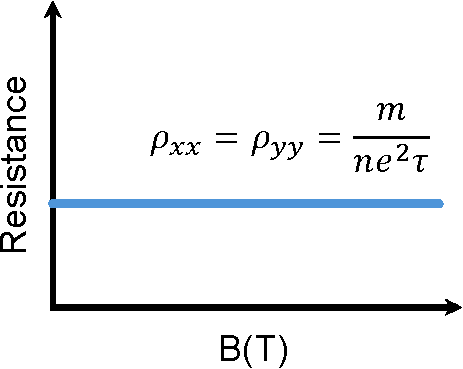
\includegraphics[width=0.75\linewidth]{pic/classRess.pdf}}
	\end{subfigure}
	\begin{subfigure}[b]{0.495\textwidth}
		\centering
		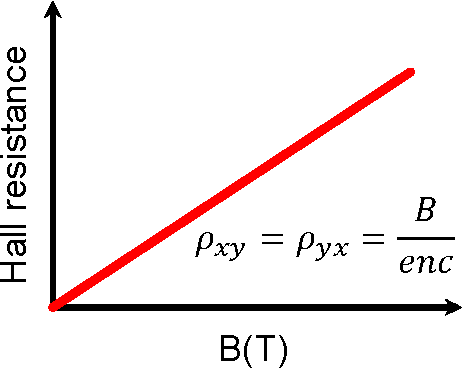
\includegraphics[width=0.75\linewidth]{pic/HallRess.pdf}
	\end{subfigure}
	\caption[Logitudinal resistance and Hall resistance plot.]{
		The longitudinal resistance on the right figure and the Hall resistance in the left figure. The graph shows both the longitudinal resistance and the Hall resistance is linear to the increasing magnetic field.
	}
\end{figure*}
\subsection{Berry curvature}
While the classical Hall effect is well explained by the Lorentz force deflecting charge carriers under a magnetic field, it fails to capture the quantized nature of Hall conductance observed in two-dimensional electron systems at low temperatures and high magnetic fields. This quantization is inherently quantum mechanical and cannot be described without considering the wavefunction topology of Bloch electrons.

In the semiclassical framework, the motion of electrons in a periodic potential acquires an additional term known as the anomalous velocity, which arises due to the Berry curvature of the Bloch bands. When an external electric field $\mathbf{E} = \left(E_{x}, E_{y}, 0\right)$ is applied, the crystal momentum $\mathbf{k}$ of the Bloch electrons become time-dependent, in accordance with the semiclassical acceleration theorem
\begin{gather}
	\hbar \dot{\mathbf{k}} = - e \mathbf{E}.
\end{gather}
The velocity of Bloch electrons is defined as
\begin{gather}
	\mathbf{v}_{\nu} = \frac{1}{\hbar} \nabla_{\mathbf{k}} \varepsilon_{\nu}(\mathbf{\mathbf{k}}) - \dot{\mathbf{k}} \times \Omega_{\nu}(\mathbf{k}),
\end{gather}
in which the second term, $ - \dot{\mathbf{k}} \times \Omega_{\nu}(\mathbf{k}) $, is known as the anomalous velocity. The Berry curvature $ \Omega_{\nu}(\mathbf{k}) $ of the $\nu$-th band is given by
\begin{gather}
	\Omega_{\nu}(\mathbf{k}) = \nabla_{\mathbf{k}} \times \Lambda_{\nu}(\mathbf{k}),
\end{gather}
where the Berry connection is defined as
\begin{gather}
	\Lambda_{\nu}(\mathbf{k}) = i \braket{u_{\nu,\mathbf{k}}}{\nabla_{\mathbf{k}} u_{\nu,\mathbf{k}}}.
\end{gather}

Substituting Eq.~(2.26) into Eq.~(2.27), we obtain the velocity for electrons of $\nu$-th band
\begin{gather}
	\mathbf{v}_{\nu}(\mathbf{k}) = \frac{1}{\hbar} \nabla_{\mathbf{k}} \varepsilon_{\nu} (\mathbf{k}) + \frac{e}{\hbar} \mathbf{E} \times \Omega_{\nu} (\mathbf{k}).
\end{gather}
The electric current density along the $x-$direction now is
\begin{equation}
	\begin{aligned}
		J_{x} &= \frac{1}{L^{2}} e \ev{v_{x}} \\
		&= \frac{e}{\hbar L^{2}} \sum_{n,\mathbf{k}} \frac{\partial \varepsilon_{n}(\mathbf{k})}{\partial k_{x}} f_{n}(\mathbf{k}) + \frac{e^{2}}{\hbar L^{2}} E_{y} \sum_{n,\mathbf{k}} \Omega_{\nu}^{z}(\mathbf{k}) f_{n}(\mathbf{k}).
	\end{aligned}
\end{equation}
Eq.~(2.31) allows us to express the Hall conductivity in terms of the Berry curvature integrated over all occupied states. This expression also implies that, if no subbands are occupied, the longitudinal conductivity vanishes, i.e., $\sigma_{xx} = 0$
\begin{gather}
	\sigma_{xy} = \f{e^{2}}{h} \sum_{n}^{\text{occ.}} \f{1}{2\pi} \dps\oiint_{\text{{BZ}}} d k_{x} d k_{y} \Omega_{\nu}^{z} (\mathbf{k}).
\end{gather}
The details derivation is given in \hyperref[appendix A]{Appendix A}.


\subsection{The Quantum Hall effect}
In Section~2.4.1, we arrived at the classical Hall resistance, which remains stable under the classical mechanics framework. However, our world is governed not only by classical physics but also by quantum mechanics. Things changes significantly at extremely low temperatures and strong magnetic fields, revealing new quantum phenomena.

There are two related phenomena which are associated to two different quantum Hall effects. These are called the \ac{IQHE} and \ac{FQHE}. In this study, we mainly focus on the \ac{IQHE} where the flux number and flux quanta are integers. This phenomenon can be understood without taking into account the Coulomb interaction between electrons, which means we shall continue using the single electron Hamiltonian that we described in \hyperref[Section 2.1]{Section 2.1}. In this section, we first discovered and subsequently understood theoretically the integer quantum Hall effect in the Hofstadter butterfly.

In two dimensional, there is a crucial relationship between the conductivity tensor $\boldsymbol{\sigma}$ and the resistivity tensor $\boldsymbol{\rho}$ is given by
\begin{equation}
	\begin{aligned}
		\begin{bmatrix}
			\sigma_{xx} & \sigma_{xy} \\
			\sigma_{yx} & \sigma_{yy}
		\end{bmatrix}
		\begin{bmatrix}
			\rho_{xx} & \rho_{xy} \\
			\rho_{yx} & \rho_{yy}
		\end{bmatrix}^{-1}
		=
		\f{1}{\rho_{xx} \rho_{yy} - \rho_{xy} \rho_{yx}}
		\begin{bmatrix}
			\rho_{yy}  & -\rho_{xy} \\
			-\rho_{yx} & \rho_{xx}
		\end{bmatrix}
	\end{aligned}.
\end{equation}
Let's take a look at the experimental data for the quantum Hall effect were perfomed in 1980 by von Klitzing \textit{et at.} \cite{klitzing90}
\begin{figure}[H]
	\centering
	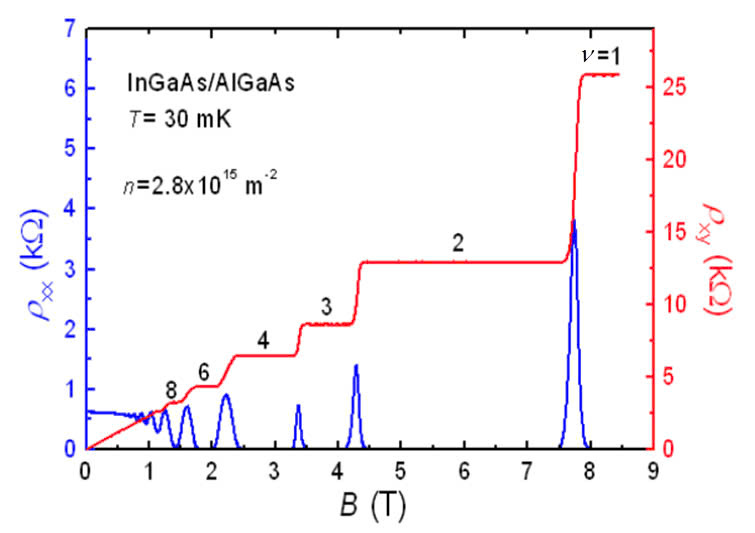
\includegraphics[width=0.7\linewidth]{pic/quantumhall.jpg}
	\caption[Quantum Hall effect by von Klitzing.]{This is the integer quantum Hall effect. For this Klaus von Klitzing was awarded the 1985 Nobel prize.}
\end{figure}
\noindent Both the Hall resistivity $\rho_{xy}$ and the longitudinal resistivity $\rho_{xx}$ depict fasinating behaviour. Perhaps the most striking feature in the figure is the fact that the Hall resistivity $\rho_{xy}$ sits on a plateau for a range of magnetic field, before jumping dramatically to the next plateau, while the longitudinal spikes sharply at the transistions between plateuax but vanishes on the plateaux themsleves. 

The Hall resistivity is now defined
\begin{gather}
	\rho_{xy} = \frac{R_{K}}{\nu}, \quad \nu = 1,2,...
\end{gather}
while $\nu$ is the total filled Landau levels and $R_{K}$ is Klitzing's resistance constant
\begin{gather}
	R_{K} = \frac{h}{e^{2}} = 25812.8074555 \Omega \pm 0.0000059 \Omega.
\end{gather}
Between two plateaux, if $\rho_{xy}  = 0$ then we get the familiar relation between resistivity and conductivity is $\sigma_{xx} = 1/\rho_{xx}$. But on these Hall plateaux
\begin{gather}
	\rho_{xy} = \rho_{yx} = \text{const} ,\; \rho_{xx} = \rho_{yy} = 0 ,
\end{gather}
this leads to
\begin{gather}
	\sigma_{xy} = \sigma_{yx} = 1 / \text{const} , \; \sigma_{xx} = \sigma_{yy} = 0.
\end{gather}
There is an apparent paradox here, we would call a system with $\rho_{xx} = 0$ is a perfect conductor, while one with $\sigma_{xx} = 0$ is a perfect insulator. But what if both $\rho_{xx} = 0$ and $\sigma_{xx} = 0$ occur simultaneously? A new material or a new state of matter?





%\subsection{Wannier diagram}
% a simplified replica of Fig, a powerful tool for visualizing the relationship between magnetic flux and electron filling in the system. Wannier's diagram provides a graphical representation of the allowed energy gaps in the Hofstadter spectruc as a function of the magnetic flux per unit cell and the electron filling factor. This diagram is particularly insightful because it captures the topological properties of the system through the distribution and behavior of these energy gaps.
%
%The fundamental of Wannier's diagram lies in the Diophantine gap equation
%\begin{gather}
%	\f{n}{n_{0}} = \nu \f{\Phi}{\Phi_{0}} + s,
%\end{gather}
%where $\frac{n}{n_{0}}$ is the electron filling factor, representing the ratio of the number of electrons per unit cell, $\nu$ is the Chern number associated with the quantized Hall conductance, and $s$ is another interg that corresponds to the gap index, effectively indicating the electron filling within the spectrum.
%
%
%
%The calculated Wannier's diagram, the energy density of state as a function of filling factor $\frac{n}{n_{0}}$ and magnetic flux $\Phi$ as illustrated in Fig, reveal the presence of these energy gaps across the spectrum. Each colored line in the diagram corresponds to an energy gap where the system exhibits an imcompressible quantumm Hall state, characterized by a quantized Hall conductance. The diagram not only provides a clear visualization of the gap structure but also offers insights into the topological phases that arise in monolayer TMD systems under varying magnetic flux conditions.
%\begin{figure}[H]
%	\centering
%	\includegraphics[width=0.8\textwidth,height=0.85\linewidth]{pic/wannier199.png}
%	\caption{Wannier diagram}
%\end{figure}

%\chapter{DISCUSSION}
%This
%\section{Result}
%\section{Discussion}
